\chapter{Architecture design} \label{ch:archdesign}
\todo{NOT DONE! rough sketch. De nedenstående trin er hvad jeg skal igennem: Para. Anal., Alloc., Optimizaiton, FSMD og VHDL + simulering }

RTL design
\section{Parallelism Analysis}

\section{Allocating / Scheduling}

\section{Optimization}

\section{FSMD design}

\section{VHDL + Simulation}

\section*{Box filter / Mean function}
\todo{this section should contain the design for my boxfilter or mean function}
As seen from the guided image filter algorithm the mean function $f_{mean}(x)$ is used multiple q

\subsection*{Finite State Machine}
\todo{beskriv FSM'en jeg har lavet (se figur 6.1) }
\begin{figure}
  \centering
  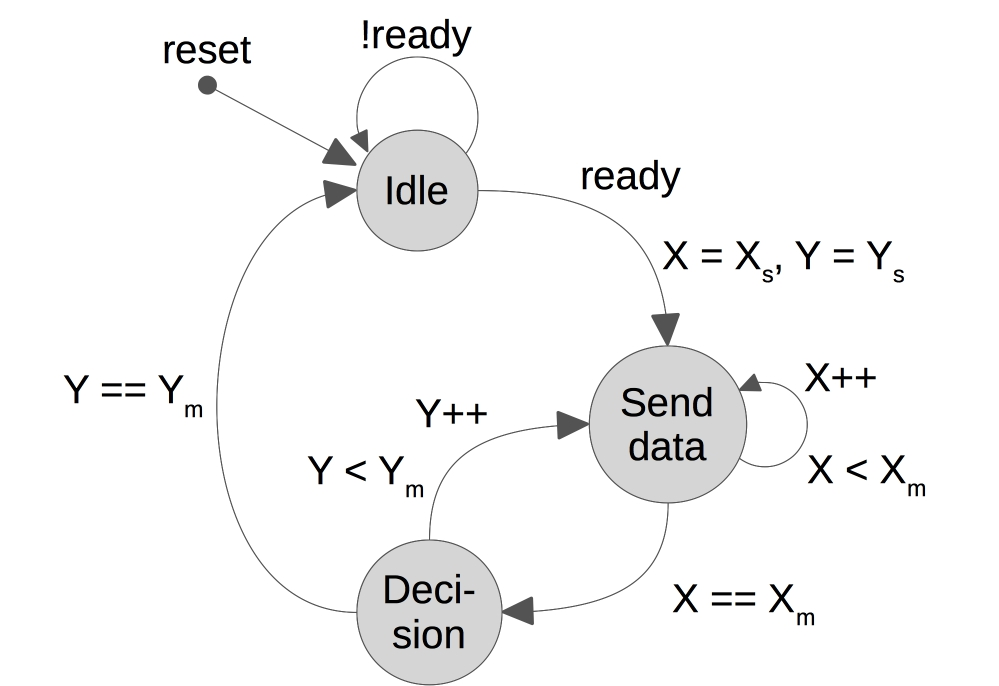
\includegraphics[width=0.5\textwidth]{figures/meanFSMv1.jpg}
  \caption{TEXT GOES HERE}
  \label{fig:LABEL}
\end{figure}

\subsection*{Memory}
\begin{figure}
  \centering
  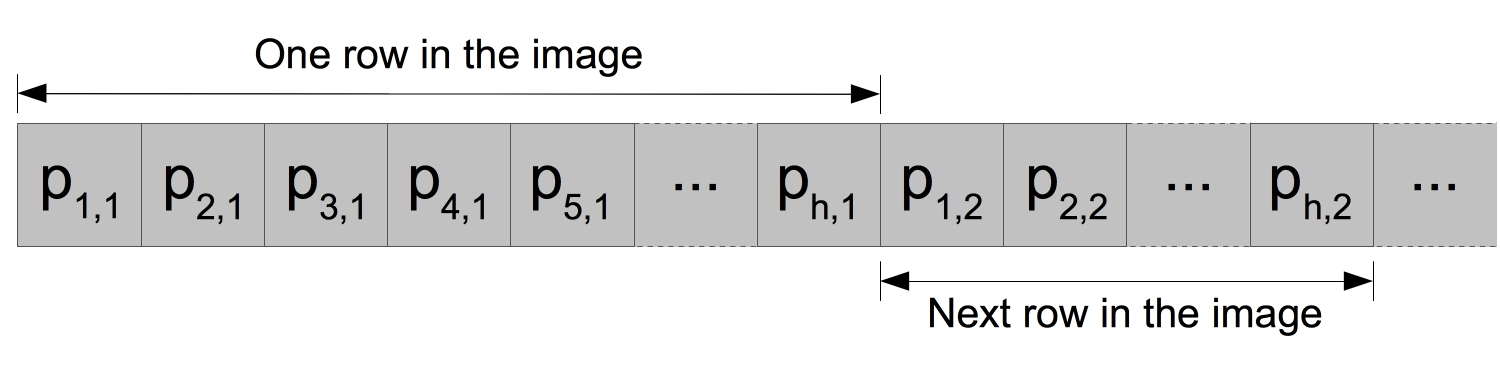
\includegraphics[width=0.5\textwidth]{figures/memdata.jpg}
  \caption{TEXT GOES HERE}
  \label{fig:LABEL}
\end{figure}

memory requirement: \\
$3 \cdot 8$ bits per pixel (rgb image). test image is $741 \times 497$ so for the test image $8.838.648$ bits $\approx$ 9 megabit $\approx$ 1.1 megabyte.

\subsection*{VHDL/Simulation}
\todo{skriv om VHDL kode og simulation af filteret}

\subsection*{Implementation/Test}
\todo{skriv om implementation på FPGA'en og gerne verificere det virker}

